% !TeX program = xelatex
% !TeX options = -shell-escape
% !TEX encoding = UTF-8

% --------------------------------------------------------------
% This is all preamble stuff that you don't have to worry about.
% Head down to where it says "Start here"
% --------------------------------------------------------------

\documentclass[12pt]{article}
\usepackage[margin=2cm]{geometry} % 頁面邊距設置
\usepackage{amsmath,amssymb,amsthm} % 數學相關套件
\usepackage{graphicx} % 圖形插入
\usepackage{booktabs} % 表格線條
\usepackage[AutoFakeBold,AutoFakeSlant]{xeCJK} % 中文支援
\usepackage{fancyhdr} % 頁首頁尾設置
\usepackage{xcolor,changepage,mdframed} % 顏色與框線相關
\usepackage{titlesec} % 標題格式
\usepackage{setspace} % 行距
\usepackage{minted} % 程式碼高亮（需安裝 Python 套件 pygments）
\usepackage[shortlabels]{enumitem} % 列表格式
\usepackage[colorlinks=true,linkcolor=black,urlcolor=blue,citecolor=blue]{hyperref} % 超連結
\graphicspath{{images}}

% 字體設定 (xeCJK)
\setCJKmainfont{黑體-繁}
\setCJKmonofont{Noto Sans CJK TC}

% 頁首/頁尾設定 (fancyhdr)
\pagestyle{fancy}
\fancyhead[L]{NASA Homework 3} % 可以用 \leftmark 取代
\fancyhead[R]{B13901011 吳亞倫}
\fancyfoot[C]{\thepage}
\renewcommand{\headrulewidth}{0.4pt}
\renewcommand{\footrulewidth}{0pt}
\setlength{\headheight}{15pt}

% tex-fmt: off
\newtheorem*{theorem}{Theorem}
\newenvironment{lemma}[2][Lemma]{\begin{trivlist}
\item[\hskip \labelsep {\bfseries #1}\hskip \labelsep {\bfseries #2.}]}{\end{trivlist}}
\newenvironment{exercise}[2][Exercise]{\begin{trivlist}
\item[\hskip \labelsep {\bfseries #1}\hskip \labelsep {\bfseries #2.}]}{\end{trivlist}}
\newenvironment{problem}[2][Problem]{\begin{trivlist}
\item[\hskip \labelsep {\bfseries #1}\hskip \labelsep {\bfseries #2}]}{\end{trivlist}}
\newenvironment{question}[2][Question]{\begin{trivlist}
\item[\hskip \labelsep {\bfseries #1}\hskip \labelsep {\bfseries #2.}]}{\end{trivlist}}
\newenvironment{corollary}[2][Corollary]{\begin{trivlist}
\item[\hskip \labelsep {\bfseries #1}\hskip \labelsep {\bfseries #2.}]}{\end{trivlist}}
\newenvironment{solution}{\begin{proof}[Solution]}{\end{proof}}
\newenvironment{answer}{\begin{proof}[Ans]}{\end{proof}}

% 樣式設定

\setminted{frame=lines, linenos, framesep=2mm, breaklines=true, breakanywhere=true, autogobble=true}

% 自訂框線環境
\newmdenv[
  linewidth=2pt, linecolor=gray, backgroundcolor=gray!10,
  topline=false, bottomline=false, rightline=false,
  skipabove=10pt, skipbelow=10pt, innerleftmargin=10pt,
  innerrightmargin=0pt, innertopmargin=5pt, innerbottommargin=5pt
]{myquote}

\newenvironment{mycolorbox}[1][gray]{
  \renewmdenv[
    linewidth=2pt, linecolor=#1, backgroundcolor=#1!10,
    topline=false, bottomline=false, rightline=false,
    skipabove=10pt, skipbelow=10pt, innerleftmargin=10pt,
    innerrightmargin=0pt, innertopmargin=5pt, innerbottommargin=5pt
  ]{myquote}
  \begin{myquote}
}{\end{myquote}}

\linespread{1.1}
% \usemintedstyle{xcode}
\AtBeginEnvironment{minted}{\vspace{-10pt}} % 可根據需求調整間距數值
\setminted{breaklines=true, breakanywhere=true, autogobble=true}

% tex-fmt: on
\begin{document}
\thispagestyle{fancy}

%------------------------------------------------------------
%                         Start here
% -----------------------------------------------------------

\begin{center}
  {\large \bfseries Network Administration / System Administration} \\
  \vspace{1em}
  {\Large \bfseries Homework 3} \\
\end{center}

\vspace{2em}

\begin{tabular}{@{}l l}
  \textbf{Student:} & 吳亞倫 \\
  \textbf{ID:} & B13901011  \\
  \textbf{Department:} & 電機工程學系
\end{tabular}
\bigskip

\begin{mycolorbox}[cyan]
  \textbf{Discussion Partners:}
  \begin{itemize}
    \item Classmates：賴泓安、鄭竣陽、陳澔樂、喻慈恩
    \vspace{0.5em}
  \end{itemize}
\end{mycolorbox}

% -----------------------------------------------------------
% Problem 1
\section{問答題}

\begin{mycolorbox}[teal]
  \textbf{Reference:}
  \begin{itemize}
    \item \href{https://www.uuu.com.tw/Public/content/article/16/160822tips.htm}{使用Cisco的Switch在區域網路裡防止ARP類型的攻擊} (Problem 1.1)
    \item \href{https://www.cisco.com/c/zh_tw/support/docs/switches/lan-switch-software/222274-troubleshoot-dynamic-arp-inspection-dai.html}{排除Catalyst交換機中的動態ARP檢測(DAI)和IP源防護故障} (Problem 1.1)
    \item \href{https://zh.wikipedia.org/zh-tw/IEEE_802.1Q}{IEEE 802.1Q} (Problem 1.2)
    \item \href{https://weihanit.wordpress.com/2017/07/27/switch%E4%B8%89%E7%A8%AEport%E6%A8%A1%E5%BC%8Faccess%E3%80%81hybrid%E3%80%81trunk%E8%A1%8C%E7%82%BA%E6%A8%A1%E5%BC%8F/}{Switch三種port模式:Access、Hybrid、Trunk} (Problem 1.2)
    \item \href{https://www.lindenphotonics.com/trunk-port-vs-access-port-understanding-the-key-differences}{Trunk Port vs Access Port: Understanding the Key Differences} (Problem 1.2)
    \item \href{https://www.netadmin.com.tw/netadmin/zh-tw/feature/0C1A2DDB3CF94296864832049D8897A4}{化繁為簡談虛擬區域網路 在Cisco交換器設定VLAN及Trunk} (Problem 1.2)
    \item \href{https://www.jannet.hk/vlan-trunking-protocol-vtp-zh-hant/}{VLAN Trunking Protocol (VTP) 虛擬區域網絡中繼協定} (Problem 1.2)
    \item \href{https://www.reddit.com/r/HomeNetworking/comments/d7lyq4/link_aggregation_not_getting_twice_the_throughput/}{Link Aggregation not getting twice the throughput} (Problem 1.3)
    \item \href{https://www.vbird.org/events/network_lacp.php}{區域網路與 switch LACP (鳥哥私房菜)} (Problem 1.3)
    \item \href{https://www.jannet.hk/spanning-tree-protocol-stp-zh-hant/}{Spanning Tree Protocol (STP) 生成樹協定} (Problem 1.4)
  \end{itemize}
\end{mycolorbox}

\subsection{DAI (Dynamic ARP Inspection)}
當在 Switch 上啟用 DAI 之後，Switch 會透過 DHCP snooping 的機制，建立一張對應真實終端機 MAC 位址與 IP 位址的表格。而當交換機收到終端主機傳來的 ARP 回應封包時，會檢查 ARP 回應封包中的 MAC 位址是否與對應表格一致，若不一致則會將此封包丟棄。這樣的機制可以有效防止 ARP spoofing 攻擊。

\subsection{VLAN 與 802.1Q}
\begin{problem}{1.2 (a)}
  當一個 port 被設定為 Access Port 時，傳入該 port 的封包基本上不包含 802.1Q 的 VLAN 標籤，因此 Switch 會將這些封包視為屬於該 port 所屬的 VLAN，並且主動加上標籤再轉發。而當一個 port 被設定為 Trunk Port 時，傳入該 port 的封包基本上都包含 802.1Q 標籤，因此 Switch 會根據標籤來決定轉發的 VLAN。若該封包不包含 VLAN 標籤，則 Switch 會將封包視為屬於 Trunk Port 所設定的 Native VLAN。
\end{problem}
\begin{problem}{1.2 (b)}
  Native VLAN 是 Trunk Port 所設定的一個預設 VLAN。當有任何沒被標記 802.1Q 標籤的封包進入 Trunk Port 時，交換器會將他視為屬於 Native VLAN 的封包。可能的使用情境是擁有某台不支援 VLAN 標記的舊設備，可以透過 Native VLAN 來正確傳送。
\end{problem}
\begin{problem}{1.2 (c)}
  VTP 讓網路管理者可以不用在每一台交換機當中都重新設定一次 VLAN。要使用 VTP 時，需要將每一台 Switch 以 truck 連接，並將其中一台設定為 VTP Server，其他設定為 VTP Client。當要修改 VLAN 設定時，只要修改 VTP server，就會自動同步到其他 VTP Client 上。
  \begin{itemize}
    \item 優點：不用重複多次設定每一台交換機，可以節省時間
    \vspace{-0.5em}
    \item 缺點：舊版本的 VTP 有安全性問題，可能會導致整個網路的 VLAN 設定被修改。另外，當 VTP Server 設定錯誤時，也可能導致整個網路都癱瘓。
  \end{itemize}
\end{problem}
\subsection{Link Aggregation}
\begin{problem}{1.3 (a)}
  Link Aggregation 可以增加連接的頻寬，但是單一連接時，還是透過單一連接的頻寬傳輸，而增加頻寬不會直接增加到信號傳輸速度。因此，當使用 Link Aggregation 時，單一連線來說傳輸速度並不會增加。
\end{problem}
\begin{problem}{1.3 (b)}
  若將一個 port 設定為 LACP 的 active 模式，則該 port 會主動發送 LACP 封包，並且會等待對方的回應。而若設定為 passive 模式，則該 port 只會等待對方的 LACP 封包，並且不會主動發送 LACP 封包。因此，在設定 Link Aggregation 時，兩端的 port 至少要有一端設為 active 模式。
\end{problem}
\begin{problem}{1.3 (c)}
  若兩端皆為 passive，則都不會主動發送 LACP 封包，因此 Link Aggregation 連接不會建立。
\end{problem}

\subsection{STP (Spanning Tree Protocol)}
\begin{problem}{1.4 (a)}
  啟用 STP 時，會以選舉方式，發送 BPDU 封包，並選擇一個 switch 作為 root switch，同時每台交換機以距離 root switch 最近的 port 為 root port，建立一顆樹。之後，交換機會將非樹邊的 port 關閉，以避免 loop 的產生。
\end{problem}
\begin{problem}{1.4 (b)}
  包含以下五種 State:
  \begin{itemize}[itemsep=0em]
    \item Disabled：Port 關閉，不會傳送或接收任何 Frame。
    \item Blocking：Port 關閉，但是會接收 BPDU Frame，以獲取 STP 的狀態。
    \item Listening：當某個 port 要啟動時，會從 Blocking 進入 Listening，並且會傳送和接受 BPDU Frame，但不會傳送 Data Frame。
    \item Learning：當 port 從 Listening 進入 Learning，會開始留意 Data frame 並學習 MAC 位址（記錄到表格），但不會傳送 Data Frame。
    \item Forwarding：Port 開啟，可以收發 BPDU 和 Data Frame。
  \end{itemize}
\end{problem}

% -----------------------------------------------------------
% Problem 2
\section{真好，又有新的 switch 可以玩了}

\begin{mycolorbox}[teal]
  \textbf{Reference:}
  \begin{itemize}
    \item \url{https://fuso002.pixnet.net/blog/post/117291204} (Problem 2.1)
    \item \href{https://david50.pixnet.net/blog/post/45217572}{Cisco 基本指令-密碼設定} (Problem 2.2)
    \item \href{https://david50.pixnet.net/blog/post/45217866}{Cisco 基本指令 - 啟用SSH} (Problem 2.3, 2.4)
    \item \url{https://ithelp.ithome.com.tw/m/articles/10185531} (Problem 2.4)
    \item \href{https://www.cloudtechadmin.com/configure-lacp-etherchannel-in-cisco-ios-switch/}{Configure LACP EtherChannel in Cisco IOS Switch} (Problem 2.7)
    \item \href{https://www.grandmetric.com/knowledge-base/design_and_configure/how-to-create-svi-interface-cisco/}{How to create SVI interface in Cisco} (Problem 2.8)
  \end{itemize}
\end{mycolorbox}

\subsection{設定 switch hostname}
以下為我的步驟：
\begin{itemize}
  \item 以 laptop1 的 terminal 連線至 switch1，修改 switch 的 hostname 為 Switch1。
  \begin{minted}[escapeinside=!!]{text}
    Switch(config)!#! hostname Switch1
    Switch1(config)!#! exit
  \end{minted}
  \item 以 laptop2 的 terminal 連線至 switch2，修改 switch 的 hostname 為 Switch2。
  \begin{minted}[escapeinside=!!]{text}
    Switch(config)!#! hostname Switch2
    Switch2(config)!#! exit
  \end{minted}
\end{itemize}

\subsection{設定 enable 指令密碼}
我在分別在兩台 switch 上的 configure terminal 中用以下指令設定加密密碼：
\begin{minted}[escapeinside=!!]{bash}
  Switch1(config)!#! enable secret enable
  Switch2(config)!#! enable secret enable
\end{minted}

\subsection{開啟 ssh 功能}
我在分別在兩台 switch 上的 configure terminal 中用以下指令開啟 ssh 功能：
\begin{minted}[escapeinside=!!]{bash}
  Switch1(config)!#! ip domain-name nasa.com
  Switch1(config)!#! ip ssh version 2
  Switch2(config)!#! ip domain-name nasa.com
  Switch2(config)!#! ip ssh version 2
\end{minted}

\subsection{設定 line vty}
我在分別在兩台 switch 上的 configure terminal 中用以下指令：
\begin{minted}[escapeinside=!!]{bash}
  Switch1(config)!#! line vty 0 4
  Switch1(config-line)!#! login local
  Switch1(config-line)!#! transport input ssh  # 開啟 ssh 連接

  Switch1(config)!#! line vty 5 15
  Switch1(config-line)!#! login local
  Switch1(config-line)!#! transport input none # 關閉全部的連接方式
\end{minted}
\vspace{-0.5cm}
\begin{minted}[escapeinside=!!]{bash}
  Switch2(config)!#! line vty 0 4
  Switch2(config-line)!#! login local
  Switch2(config-line)!#! transport input ssh  # 開啟 ssh 連接

  Switch2(config)!#! line vty 5 15
  Switch2(config-line)!#! login local
  Switch2(config-line)!#! transport input none # 關閉全部的連接方式
\end{minted}

\subsection{設定 VLAN}
我使用以下指令設定 VLAN：
\begin{minted}[escapeinside=!!]{bash}
    Switch1(config)!#! vlan 10
    Switch1(config-vlan)!#! name VLAN10

    Switch1(config)!#! vlan 20
    Switch1(config-vlan)!#! name VLAN20

    Switch1(config)!#! vlan 99
    Switch1(config-vlan)!#! name VLAN99
  \end{minted}
    \begin{minted}[escapeinside=!!]{bash}
      Switch2(config)!#! vlan 10
      Switch2(config-vlan)!#! name VLAN10
  
      Switch2(config)!#! vlan 20
      Switch2(config-vlan)!#! name VLAN20
  
      Switch2(config)!#! vlan 99
      Switch2(config-vlan)!#! name VLAN99
    \end{minted}

\subsection{Port 設定}
設定 Switch1 port 的指令：
  \begin{minted}[escapeinside=!!]{bash}
    Switch1(config)!#! interface FastEthernet 0/1
    Switch1(config-if)!#! switchport mode access
    Switch1(config-if)!#! switchport access vlan 10

    Switch1(config)!#! interface FastEthernet 0/2
    Switch1(config-if)!#! switchport mode access
    Switch1(config-if)!#! switchport access vlan 20

    Switch1(config)!#! interface FastEthernet 0/3
    Switch1(config-if)!#! switchport mode access
    Switch1(config-if)!#! switchport access vlan 99
  \end{minted}
  設定 Switch2 port 的指令：
    \begin{minted}[escapeinside=!!]{bash}
      Switch2(config)!#! interface FastEthernet 0/4
      Switch2(config-if)!#! switchport mode access
      Switch2(config-if)!#! switchport access vlan 10
  
      Switch2(config)!#! interface FastEthernet 0/5
      Switch2(config-if)!#! switchport mode access
      Switch2(config-if)!#! switchport access vlan 20  
    \end{minted}
\vspace{-0.5cm}
\subsection{設定 Switch1 和 Switch2 之間的的連接}
使用 Lab4 簡報上的指令，可以完成題目要求：
\begin{minted}[escapeinside=!!]{bash}
  Switch1(config)!#! interface range GigabitEthernet 0/1-2
  Switch1(config-if-range)!#! channel-group 1 mode active
  Switch1(config-if-range)!#! channel-protocol lacp
  Switch1(config)!#! interface port-channel 1
  Switch1(config-if)!#! switchport mode trunk
  Switch1(config-if)!#! switchport trunk allowed vlan 10,20,99
\end{minted}
\vspace{-0.5cm}
\begin{minted}[escapeinside=!!]{bash}
  Switch2(config)!#! interface range GigabitEthernet 0/1-2
  Switch2(config-if-range)!#! channel-group 1 mode active
  Switch2(config-if-range)!#! channel-protocol lacp

  Switch2(config)!#! interface port-channel 1
  Switch2(config-if)!#! switchport mode trunk
  Switch2(config-if)!#! switchport trunk allowed vlan 10,20,99
\end{minted}

\subsection{管理者帳號}
建立管理者帳號：
\begin{minted}[escapeinside=!!]{bash}
  Switch1(config)!#! username admin privilege 15 secret nasa2025
  Switch2(config)!#! username admin privilege 15 secret nasa2025
\end{minted}
設定 svi 介面：
\begin{minted}[escapeinside=!!]{bash}
  Switch1(config)!#! interface vlan 99
  Switch1(config-if)!#! ip address 192.168.99.1 255.255.255.0
  Switch1(config-if)!#! no shutdown
  
  Switch2(config)!#! interface vlan 99
  Switch2(config-if)!#! ip address 192.168.99.2 255.255.255.0
  Switch2(config-if)!#! no shutdown
\end{minted}
\clearpage
% -----------------------------------------------------------
% Problem 3
\section{你在 switch 上玩什麼！}

\begin{mycolorbox}[teal]
  \textbf{Reference:}
  \begin{itemize}
    \item \href{https://zh.wikipedia.org/zh-tw/%E7%AE%80%E5%8D%95%E7%BD%91%E7%BB%9C%E7%AE%A1%E7%90%86%E5%8D%8F%E8%AE%AE}{簡單網路管理協議 (Wikipedia)}
    \item \href{https://www.manageengine.com/tw/network-monitoring/what-is-snmp.html#snmp-version}{SNMP 教程}
    \item \href{https://www.cisco.com/c/en/us/td/docs/ios-xml/ios/snmp/configuration/xe-16/snmp-xe-16-book/nm-snmp-cfg-snmp-support.html#GUID-D77A13E8-EFF6-435E-BB74-1BBBB390901B}{SNMP Configuration Guide}
  \end{itemize}
\end{mycolorbox}

\subsection{SNMP} 
  SNMP 是一個協定，他允許管理者監控網路設備的狀態，以及那些設備有沒有做出異常的行為。在被管理的設備上，會有一個稱之為 agent 的軟體，他會定期的將設備的狀態資訊傳送給管理者。SNMPv3 相比 SNMPv2，強化了安全性以及遠端組態的管理，包含加上加密以及認證等等。
\subsection{MIB}
  MIB (Management Information Base) 是 SNMP 用來儲存網路中裝置資訊的資料庫。SNMP 管理者可以來查詢這些物件的值，作為回應 agent 請求的依據。
\subsection{監控 MIB 項目}
我認為可以監控以下項目：
\begin{itemize}
  \item \texttt{ifInOctets / ifOutOctets}：可以監控網路流量，當突然封包數量大幅增加時，極有可能是網路阻塞了。
  \item \texttt{ifInErrors / ifOutErrors}：檢查網路介面的錯誤數量，當錯誤數量增加時，可以辨識是否有網路阻塞現象
  \item \texttt{cpmCPUTotal5sec / cpmCPUTotal1min / cpmCPUTotal5min / cpmCPUMemoryUsed}：用來監控交換機的 CPU 使用率，可以及時得知是否 CPU 使用率過高，導致網路阻塞。
\end{itemize}

\subsection{模擬監控}
在 Switch0 的 CLI 中：
\begin{minted}{text}
  Switch0(config)# snmp-server community public ro
  Switch0(config)# snmp-server community private rw
  Switch0(config)# exit
  Switch0# write memory
\end{minted}
之後，在跟隨指示操作，在 PC0 > Desktop > MIB Browser > Advanced 當中， Read Community 輸入 public， Write Community 輸入 private，並且輸入 Switch0 的 IP 位址。最後，在 OID 欄位輸入 \texttt{.1.3.6.1.2.1.1.5.0}，即可查詢到 hostname。結果如下圖所示。
\begin{figure}[H]
  \centering
  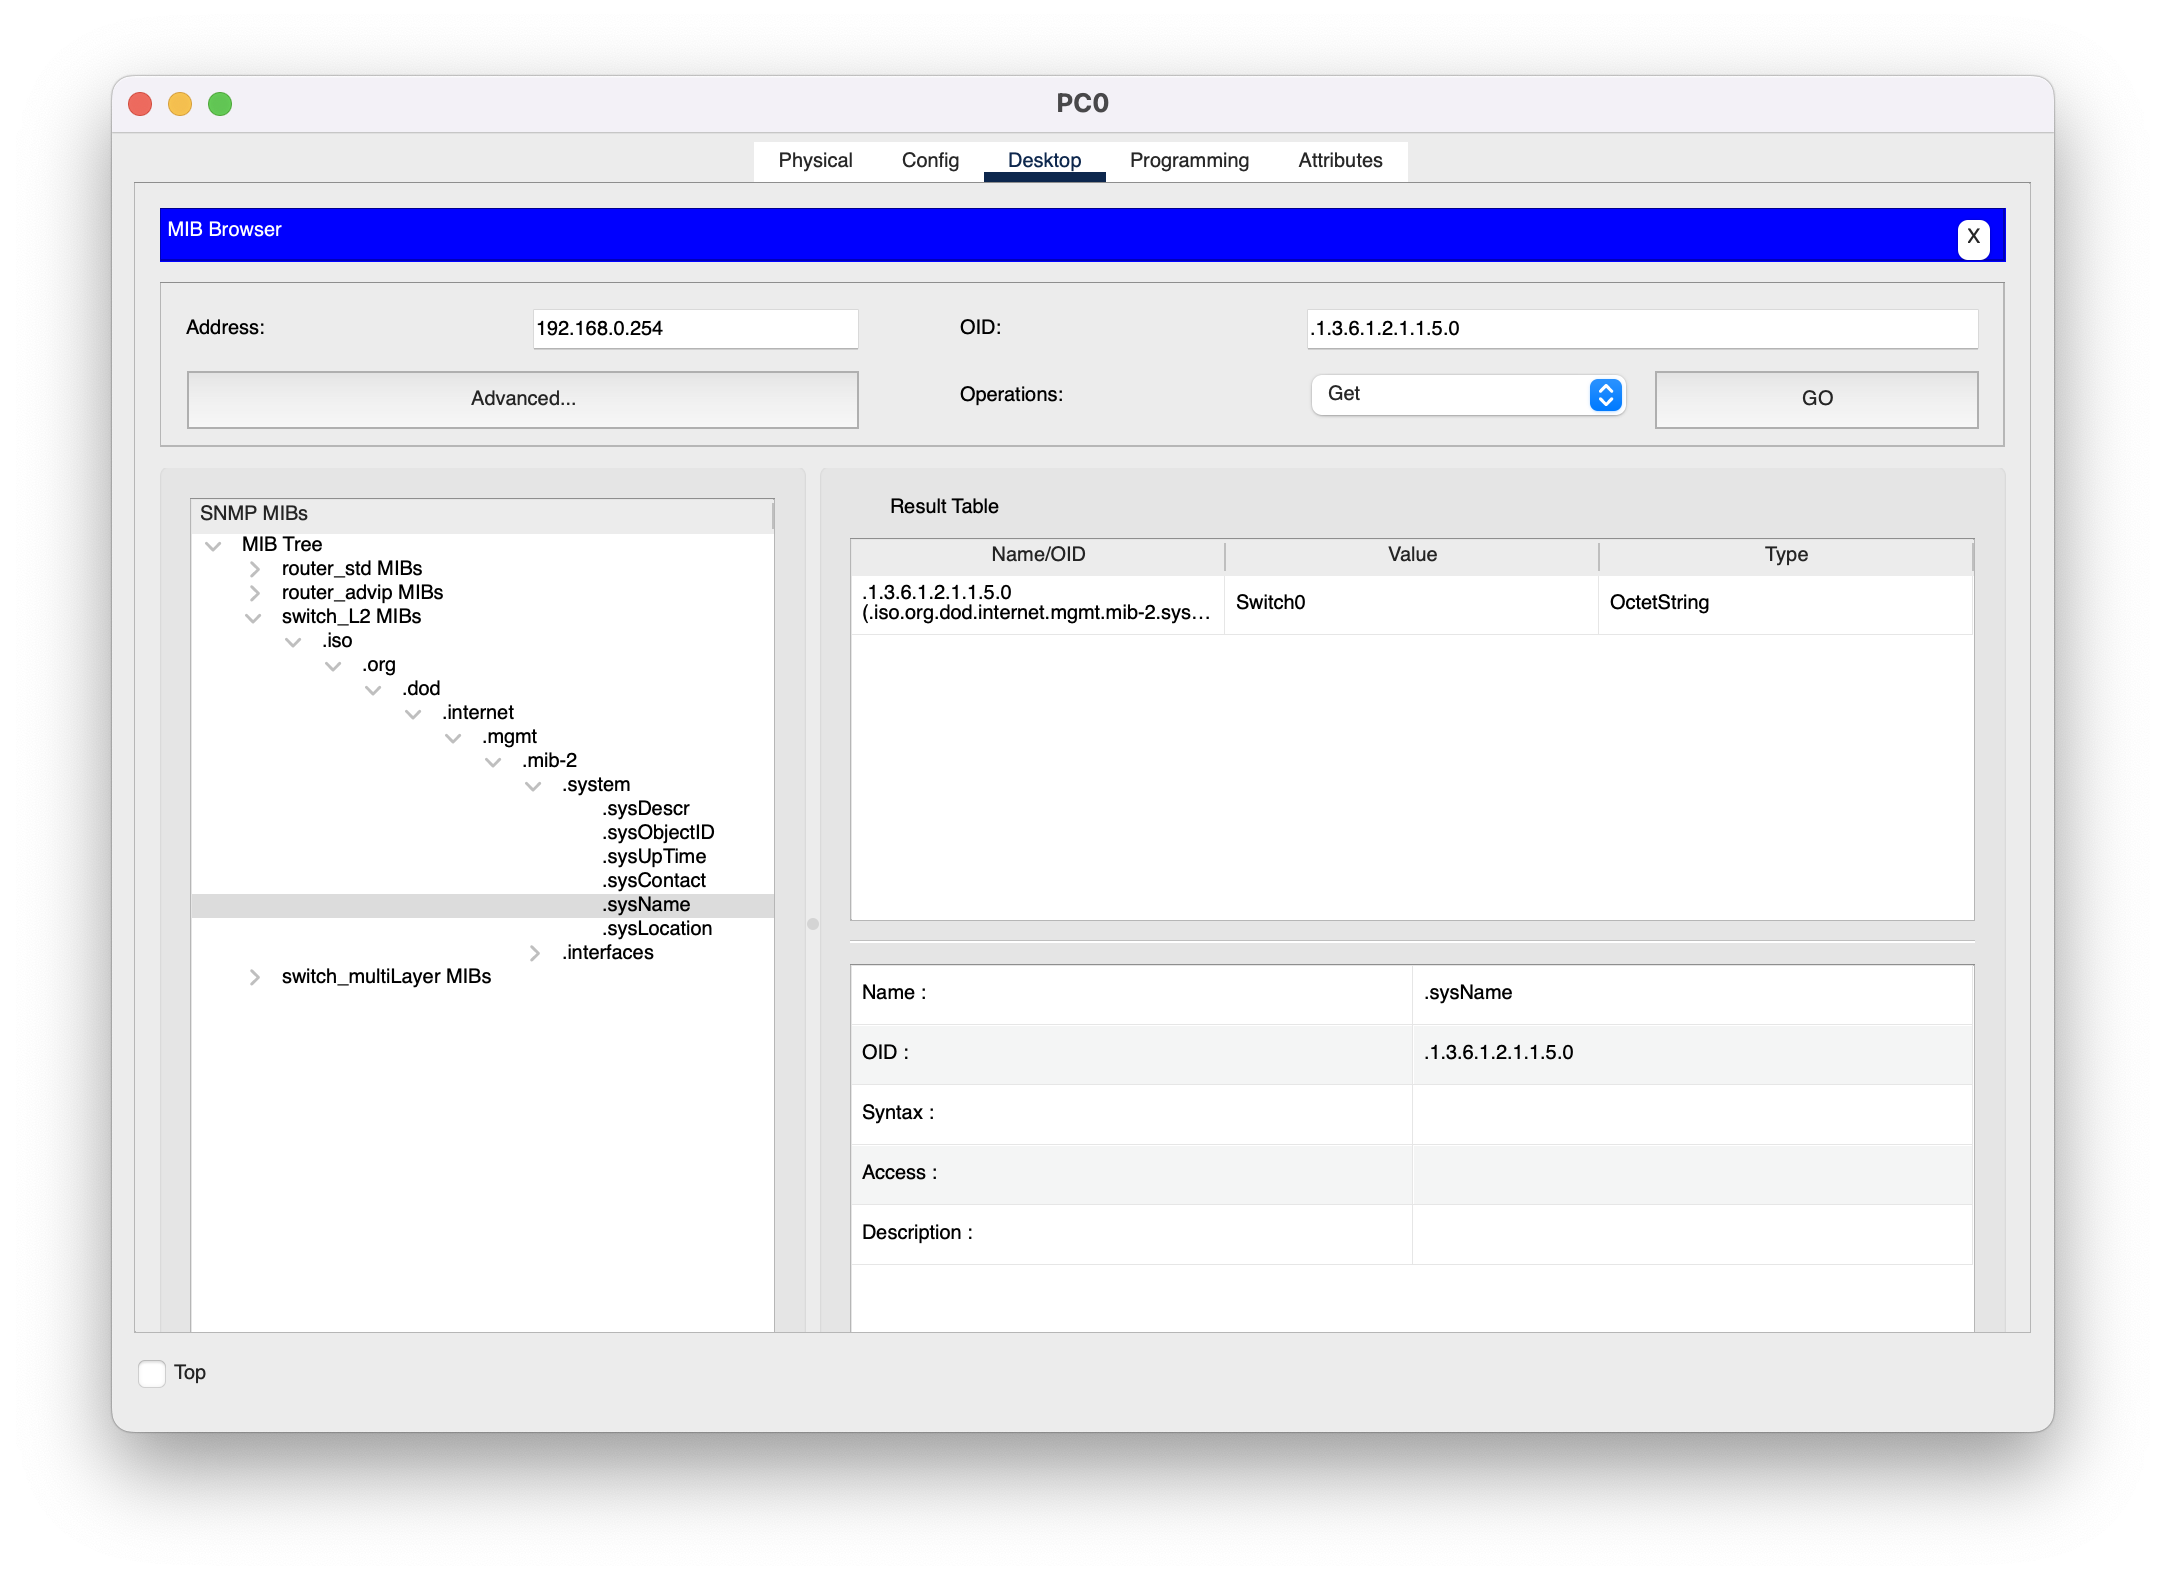
\includegraphics[width=\textwidth]{images/3-4-1.png}
  \label{fig:3-4-1}
  \caption{結果截圖}
\end{figure}
% -----------------------------------------------------------
%    You don't have to mess with anything below this line.
% -----------------------------------------------------------

\end{document}
